\section{Proposed Method}\label{method}

\begin{figure}
\centering
\begin{tabular}{cc}
      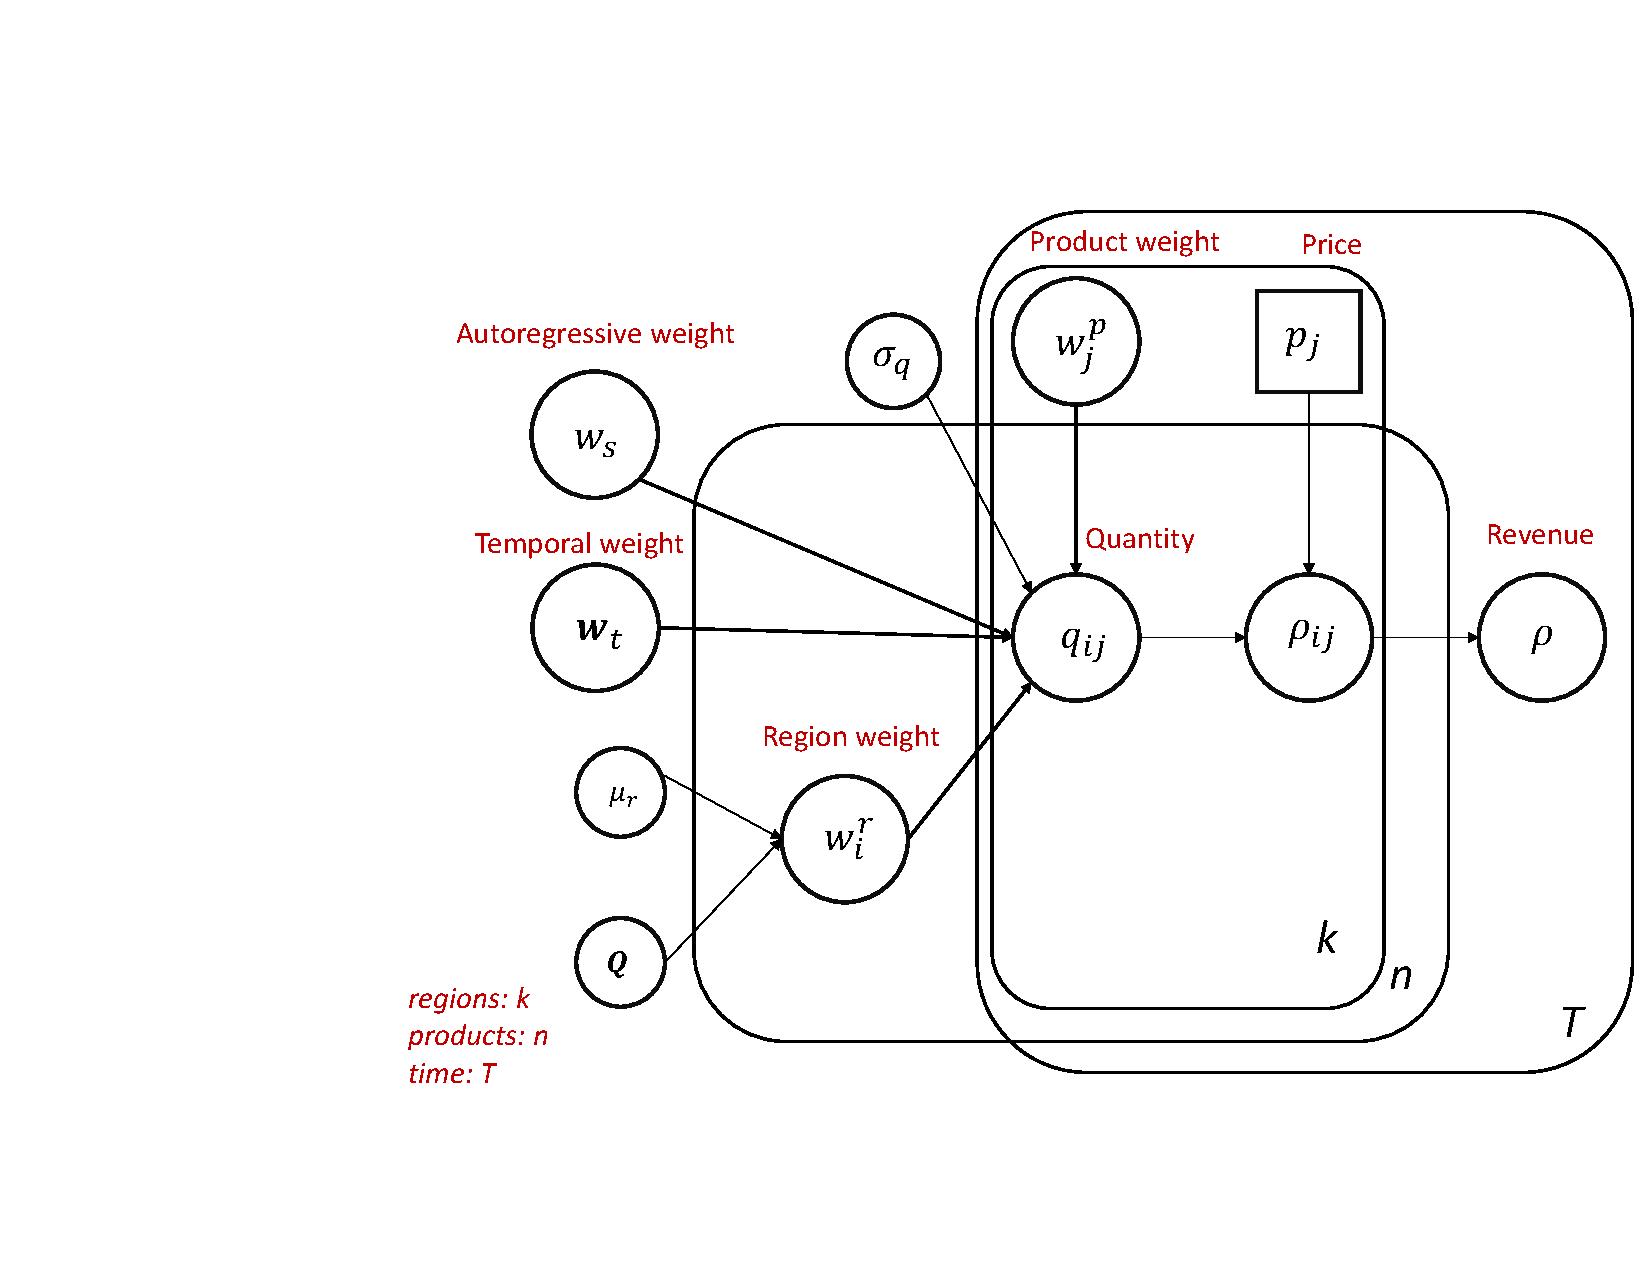
\includegraphics[scale=.35]{figs/model-linear.pdf}
\end{tabular}
    
   
\caption{An overview of the proposed model as a Bayesian network. The boxes are ``plates'' representing structures in the data. The plates marked by $k$, $n$ and $T$ represent products, regions, and time, respectively.  Circles denote random variables and squares are deterministic quantities. The model decomposes quantity as a function of region, product, time, and auto-regressive weights.}
\label{model-fig}
\end{figure}

In this section, we define our framework for solving the optimal allocation problem. Specifically, we outline our proposed environment model that is used to simulate spatial demand. 


\subsection{Stochastic Model of Spatial Demand}\label{simple-model}

We propose the following stochastic model of spatial demand in physical retail. See Figure \ref{model-fig} for an overview. In the current work, the stochastic model is used as a `simulator' to enable offline policy learning. There are many advantages of using a probabilistic model in the optimal product allocation problem. First, we are able to incorporate prior knowledge about the data generating process, which can again improve data efficiency and model effectiveness. Second, it provides a natural framework for simulating future scenarios through Monte Carlo roll-outs.

Our ultimate objective is to maximize total revenue at time, $\rho^{(t)}$, which is defined as:

\begin{equation}
    \rho^{(t)} =  \sum_{i=1}^n \rho_i^{(t)}
\end{equation}

where $\rho_i^{(t)}$ is the revenue for region, $r_i$. Region-level revenue is calculated over products, $m_j$:

\begin{equation}
    \rho_i^{(t)} = \sum_{j=1}^k p_j q_{ij}^{(t)}
\end{equation}

The key variable of interest is, $q_{ij}^{(t)}$, the quantity sold for product, $m_j$, region, $r_i$, at time, $t$. We model  $q_{ij}^{(t)}$ as a truncated normal random variable:

\begin{equation}
    q_{ij}^{(t)} \sim \psi(\mu, \sigma, a, b)
\end{equation}


where, $\psi(\mu, \sigma, a, b)$ is the pdf of the truncated normal distribution. The term, $\phi(z)$ is the standard normal pdf, and $\Phi(z)$ is its cumulative distribution function. See \cite{Burkardt} for more details. We set $a = 0$ and $b=+\infty$, which forces $\Phi(\mu, \sigma^2; b) = 1$ and constrains quantity, $ q_{ij}^{(t)} \in \mathbb{R}^{+}$. The prior for $ q_{ij}^{(t)}$ is characterized by the mean, $\mu_q$, which is a linear function of environment features, $\textbf{x}$ and learned weights, $\textbf{w}$, and the inverse gamma distribution for the variance, $\sigma_q$:

\begin{equation}
    \mu_q = \textbf{x}^{\top}\textbf{w} + b
\end{equation}

\begin{equation}
    \sigma_q \sim \text{IG}(\alpha_q, \beta_q)
\end{equation}


In our environment, we observe temporal features, $\textbf{x}_t$,  region features, $\textbf{x}_r$, product features, $\textbf{x}_p$, and autoregressive features, $\textbf{x}_s$: \textbf{x} = $[\textbf{x}_t, \textbf{x}_r, \textbf{x}_p, \textbf{x}_s]^{\top}$. We discuss our feature extraction approach more in section \ref{features}


\subsubsection{Region-level Weights}
We initially model the weights for each spatial region with a multivariate normal distribution, with mean vector, $\boldsymbol{\mu}_r$ and covariance matrix, $\textbf{Q}_r$:

\begin{equation}\label{simple-w-r}
    \textbf{w}_r \sim \mathcal{N}(\boldsymbol{\mu}_r, \textbf{Q}_r)
\end{equation}

\subsubsection{Product-level Weights}

We also define weights for each product, $m_j$, as follows:

\begin{equation}
    \textbf{w}_p \sim \mathcal{N}(\boldsymbol{\mu}_p, \boldsymbol{\Sigma}_p)
\end{equation}

\begin{equation}
    \boldsymbol{\mu}_p \sim \mathcal{N}(\boldsymbol{\delta}_p, \boldsymbol{\Gamma}_p)
\end{equation}

\begin{equation}
    \boldsymbol{\Sigma}_p = \textbf{L}\textbf{L}^{\top} \sim \text{LKJ}(\sigma_p)
\end{equation}


We put a multivariate normal prior over the mean vector, $\boldsymbol{\mu}_p$ which has hyperparameters $\boldsymbol{\mu}_t$ and $\boldsymbol{\Sigma}_t$. Additionally, we put an LKJ prior over the covariance matrix, $\boldsymbol{\Sigma}_p$. We reparameterize $\boldsymbol{\Sigma}_t$ as its cholesky decomposition, $\textbf{L}\textbf{L}^{\top}$, so that the underlying correlation matrices follows an LKJ distribution \cite{lewandowski}. The standard deviations, $\sigma_p$, follow a half-cauchy distribution. The advantage of the LKJ prior is that is more computationally tractable than other covariance priors \cite{lewandowski}.


\subsubsection{Temporal weights}
 The temporal features capture the long-term and short-term seasonality of the environment. The temporal weights are defined similar to the product weights. Namely, the temporal weights, $\textbf{w}_t$, follow a multivariate normal distribution, with a normal prior over the mean, and the LKJ prior for the covariance matrix:

\begin{equation}
    \textbf{w}_t \sim \mathcal{N}(\boldsymbol{\mu}_t, \boldsymbol{\Sigma}_t)
\end{equation}

\begin{equation}
    \boldsymbol{\mu}_t \sim \mathcal{N}(\boldsymbol{\delta}_t, \boldsymbol{\Gamma}_t)
\end{equation}

\begin{equation}
    \boldsymbol{\Sigma}_t = \textbf{L}\textbf{L}^{\top} \sim \text{LKJ}(\sigma_t)
\end{equation}



\subsubsection{Autoregressive weight}
Finally, we specify the weight of previously observed revenue values on $q_{ij}^{(t)}$. The feature, $\textbf{x}_s$ is an autoregressive feature denoting the previous k values of product-level revenue, $\rho_j^{t} =  \sum_{j=i}^n p_j q_{ij}^{(t)}$. We assume truncated normal prior for $w_s$, and half cauchy priors for the location, $\mu_s$ and scale, $\sigma_s$:

\begin{equation}
    w_s \sim  \psi(\mu_s, \sigma_s, a, b)
\end{equation}

\begin{equation}
    \mu_s \sim \text{HalfCauchy}(\phi_s)
\end{equation}

\begin{equation}
    \sigma_s \sim \text{HalfCauchy}(\psi_s)
\end{equation}


We again set $a = 0$ and $b=+\infty$ such that $\textbf{w}_s \in \mathbb{R}^{+}$. 




\begin{equation}\label{heterogenous-w-r}
    \textbf{w}_{ij}^r \sim \mathcal{N}(\textbf{w}_r, \textbf{Q}_r)
\end{equation}

\begin{equation}
    \textbf{w}_r \sim \mathcal{N}(\boldsymbol{\mu}_i, \textbf{Q}_r)
\end{equation}

Note that both $\textbf{w}_r$ and $\textbf{w}_{ij}^r$ share the same same covariance structure. Thus, the region weights are only hierarchical in their means. Additionally, we treat the upper-level mean vector, $\boldsymbol{\mu}_r$ as hyperparameter. In Section \ref{experiments} we test which environment model is more effective at predicting revenue on a test set.


\subsection{Training} We train the proposed model using the No U-Turn Sampler (NUTS) algorithm \cite{nuts}. This allows us to draw samples from the posterior distribution of model weights, $\textbf{W}$, as well as the posterior predictive distribution of quantity, $q_{ij}^{(t)}$, and revenue $\rho^{(t)}$. We use Automatic Differention Variational Inference (ADVI) \cite{advi} as an initialization point for the sampling procedure. All models are implemented in PyMC3 \cite{pymc3}

We initialize with ADVI using 200,000 iterations. Once initialized, we sample the posterior using NUTS with a tuning period of 5,000 draws followed by 5,000 samples across four chains.


\subsection{Feature Extraction}\label{features}
In order to train the proposed model, we extract environment-level features, $\textbf{x}$, which is composed of temporal features, $\textbf{x}_t$,  region features, $\textbf{x}_r$, product features, $\textbf{x}_p$, previous sales features and $\textbf{x}_s$.

\begin{itemize}
    \item \textbf{Temporal features} We use a one-hot vector denoting the day of the week for, $\textbf{x}_t$. This feature vector captures the short-term temporality commmon in physical retail settings. For example, weekends tend to be busier shopping days than weekdays. 
    \item \textbf{Region features} We again use a one-hot vector for spatial regions, $\textbf{x}_r$. This feature vector 'turns on' the weight that each region has on quantity via the weight vector, $\textbf{w}_r$.
    \item \textbf{Product features} We expect each product to vary in popularity. We capture this effect by constructing a one-hot vector for products, $\textbf{x}_p$.
    \item \textbf{Previous sales features} Finally, we construct an autoregressive sales feature that represents the sales at time, $t-1$. We use the previous sales for product $m_j$, summed across all regions, $w_s = \rho_j^{(t-1)} = \sum_{i=1}^k p_j q_{ij}^{(t-1)}$. This feature captures micro-fluctuations in demand for each product. 
\end{itemize}


